% Chapter 13 (English edition) -- ED-14: reproduction and audit of the claimed Sandier--Serfaty proof (no proof claimed)
% Translated from papers/discovery_journal_2026/chapters/c13.tex. Figure: code/fig13.py.
\chapter[Redoing someone else's calculation]{Redoing someone else's calculation, without declaring it right}

\reference{Published on 26 October 2026. doi:10.5281/zenodo.23653827}

\section*{The idea in one picture}

Place electric charges of the same sign on an infinite plane, and spread underneath a perfectly
uniform ``paste'' of opposite charge that balances the whole. How do the charges arrange
themselves so that the energy is as low as possible? In 2012, two mathematicians conjectured
that the answer is, once again, the triangular lattice. This is known as the Sandier--Serfaty
conjecture.

In September 2026, a manuscript in the openai/math collection, produced by an AI and not
reviewed by peers, claims to give a proof of it: a mathematical reduction to a smaller problem,
then a long exact computer calculation, a ``certificate'', that checks inequalities on very fine
grids of points. Before anyone relies on it, it had to be looked at closely. \textbf{This chapter
does not say that the conjecture is proved. The work described here does not prove it, does not
verify it and does not refute it, and it is not a peer review.}

\begin{analogie}
Someone you do not know hands you an addition of a thousand lines and their reasoning. You run
their calculator again at home, with the same program; you slip in an error on purpose to see
whether it complains; and you read the reasoning line by line. \emph{Where the picture stops:}
it is the same program, not a second, independent calculator. If a formula coded inside it is
wrong, running it again reproduces the error exactly. And reading is not approving.
\end{analogie}

\section*{What was done}

Three things. \emph{First, the reproduction}: the certificate's program, unchanged, was
recompiled and rerun on another machine, with other versions of the tools. It finished in
478~seconds, about eight minutes, answering ``OK'', and the 22 pairs of integers it prints are
identical to those of the original record. Then it was sabotaged in three ways, loosening a
single constant each time. Two sabotages were rejected by the program itself; the third gets
through. For the last two, the outcome had been predicted in writing before the computation
finished. This shows where the certificate has some slack and where it has hardly any: one
constant can be multiplied by about 22, another by less than 2 only (these thresholds are fitted
after the fact, not predicted).

\emph{Then the reading}: an AI agent redid, step by step, the 31 numbered steps of the
reduction and compared the 14 steps of the program with the inequalities they are meant to
establish. No step was classified as a gap, within the limits stated below.

\emph{Finally, a Lean statement}: the conjecture was written in the Lean language as an
\emph{unproved} claim. Ten small lemmas only check that the statement is not empty of meaning.

\begin{encadre}
\textbf{To do with a pencil: a calibration check.} The certificate prints three numbers, called
$\lambda\approx-6.73003$, $\mu\approx0.4138834$ and $K\approx-0.003482$. An exact identity from
the manuscript says that $6K+\lambda+2\pi\mu$ must equal the energy of the triangular lattice,
$W\approx-4.150413$. Compute: $6K\approx-0.02089$, $2\pi\mu\approx2.60051$, and
$-6.73003-0.02089+2.60051=-4.15041$. It fits. But beware: this test is \emph{blind} to
$\lambda$ and $\mu$, which cancel each other exactly in it. So they were also recomputed
separately, from the manuscript's formulas alone, with 45 digits.
\end{encadre}

\section*{How we made sure it is not wrong}

The three pieces are not of the same level, and the paper does not mix them.
The reproduction is \niveau{X} \emph{a pencil sketch}: it is an exact calculation on integers,
but redone by the same program, and the paper files it at the sketch level. The reading of the
reduction is \niveau{C}: reasoning, carried out here by an AI and not by a human, that nobody has
verified by machine. The ten lemmas are \niveau{A} \emph{the judge has looked}: the Lean kernel checked them, axioms
within the short list, planted false proofs exposed, and the module was replayed without error on
26 October 2026, after the paper was published.\reference{Replay of 26 October 2026,
\nolinkurl{results/kernel_replay_2026-10-26/replay.jsonl}, line 86: module
\nolinkurl{Programmes.SandierSerfatyStatement}, exit code~0.} These lemmas only say that the
statement is not empty of meaning; they prove nothing about the conjecture.

A second agent, from the same AI pipeline, audited the whole. It recompiled the Lean files,
traced every number back to its file, redid calculations by another route, and returned the
verdict ``accept with corrections'', with three required corrections: a badly printed number (a
residual of $10^{-53}$ displayed as if it were $-1$), a sentence that asserted a conclusion
instead of stating it under a condition, and above all a \emph{hole in the in-house tool}: the
project's Lean file checker could be fooled by a file that stops before the verification and
prints a false report. The hole has been plugged, with tests. No human has read this work.

\section*{What this does not say}

\begin{limite}
\begin{itemize}
\item \textbf{Nothing is proved} about the conjecture. Everything that rests on the OpenAI
  manuscript remains conditional on that manuscript.
\item The reproduction relies on the manuscript's analytic bounds and tests none of them.
\item Some parts of the program were only read in the code; no sabotage reaches the last step;
  the internal proofs of the quoted results were not redone.
\item ``No gap found'' means that the agent did not see one, not that there is none.
\end{itemize}
\end{limite}

\section*{Going further}

The paper (14 pages): doi:10.5281/\allowbreak zenodo.23653827. The sequel, having the Lean judge
itself redo part of the certificate, is in doi:10.5281/\allowbreak zenodo.23656804.

\begin{figure}[ht]
\centering
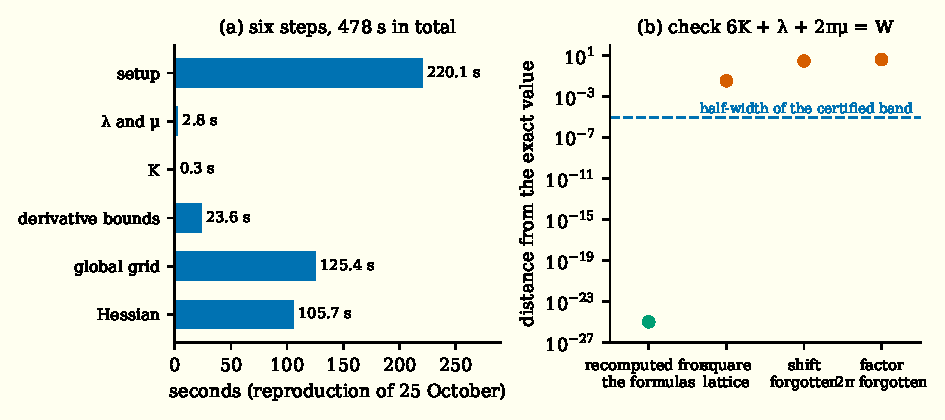
\includegraphics[width=\linewidth]{figures/c13_reproduction}
\caption{(a) Duration of the six steps during the reproduction. (b) The recomputation falls inside the certified band; the false controls fall outside it.}
\end{figure}
